\documentclass[tikz,border=8pt]{standalone}
\usepackage{tikz}
\usepackage{pgfplots}
\usepackage{amsmath,amssymb}
\usepackage[T1]{fontenc}
\usepackage{lmodern}
\usepackage{xcolor}
\usetikzlibrary{arrows.meta,positioning,shapes.geometric,fit,calc,backgrounds,matrix}
\pgfplotsset{compat=1.18}
\definecolor{ink}{HTML}{18202A}
\definecolor{blue}{HTML}{2563EB}
\definecolor{bluefill}{HTML}{EAF1FF}
\definecolor{green}{HTML}{14804A}
\definecolor{greenfill}{HTML}{E8F6EE}
\definecolor{amber}{HTML}{B56A00}
\definecolor{amberfill}{HTML}{FFF3D6}
\definecolor{red}{HTML}{B42318}
\definecolor{redfill}{HTML}{FDECEC}
\definecolor{gray}{HTML}{667085}
\definecolor{light}{HTML}{F4F6F8}
\definecolor{linegray}{HTML}{C7CDD4}
\tikzset{
  box/.style={draw=ink, rounded corners=3pt, very thick, fill=white, align=center, inner sep=7pt, font=\sffamily\small},
  bluebox/.style={box, fill=bluefill, draw=blue},
  greenbox/.style={box, fill=greenfill, draw=green},
  amberbox/.style={box, fill=amberfill, draw=amber},
  redbox/.style={box, fill=redfill, draw=red},
  ghost/.style={draw=linegray, rounded corners=3pt, thick, fill=light, align=center, inner sep=7pt, font=\sffamily\small},
  label/.style={font=\sffamily\footnotesize, text=gray, align=center},
  title/.style={font=\sffamily\bfseries\large, text=ink, align=center},
  arrow/.style={-{Latex[length=3mm,width=2mm]}, very thick, draw=ink},
  bluearrow/.style={-{Latex[length=3mm,width=2mm]}, very thick, draw=blue},
  redarrow/.style={-{Latex[length=3mm,width=2mm]}, very thick, draw=red},
  greenarrow/.style={-{Latex[length=3mm,width=2mm]}, very thick, draw=green}
}

\begin{document}
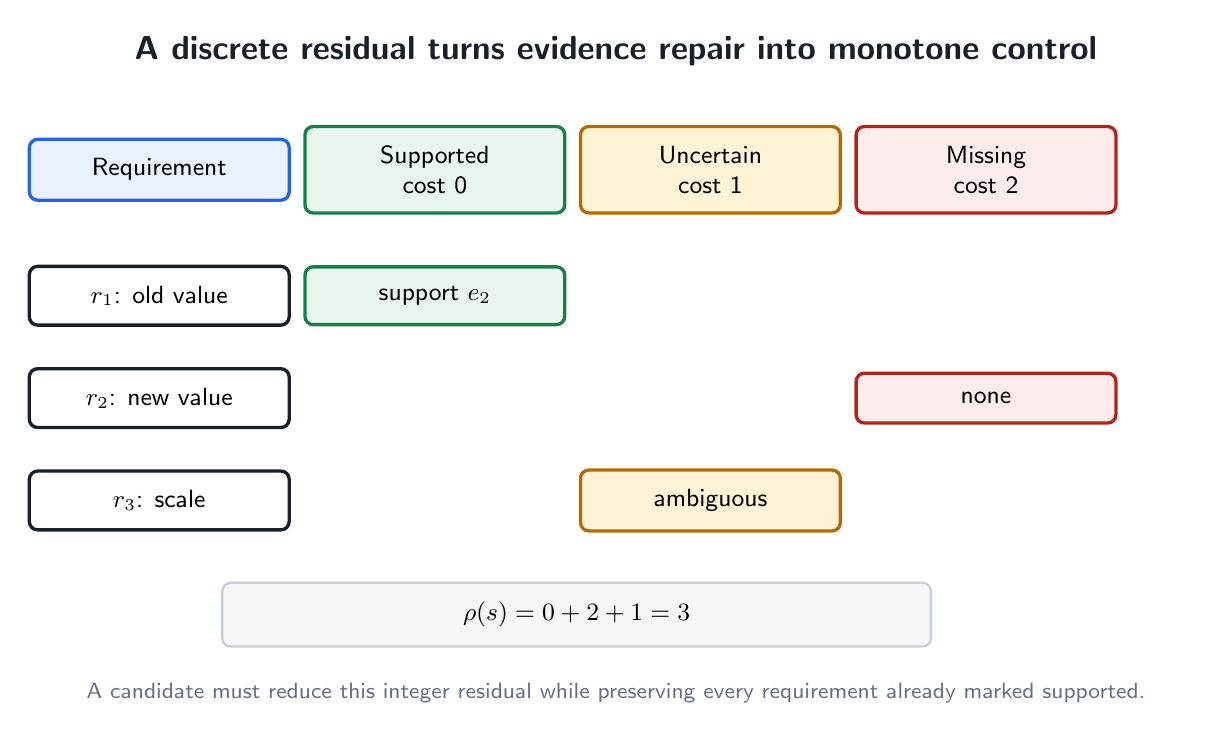
\begin{tikzpicture}
\node[title] at (7.5,5.6) {A discrete residual turns evidence repair into monotone control};
\node[bluebox, minimum width=33mm] at (1.7,4.1) {Requirement};
\node[greenbox, minimum width=33mm] at (5.2,4.1) {Supported\\cost 0};
\node[amberbox, minimum width=33mm] at (8.7,4.1) {Uncertain\\cost 1};
\node[redbox, minimum width=33mm] at (12.2,4.1) {Missing\\cost 2};
\node[box, minimum width=33mm] at (1.7,2.5) {$r_1$: old value};
\node[greenbox, minimum width=33mm] at (5.2,2.5) {support $e_2$};
\node[box, minimum width=33mm] at (1.7,1.2) {$r_2$: new value};
\node[redbox, minimum width=33mm] at (12.2,1.2) {none};
\node[box, minimum width=33mm] at (1.7,-0.1) {$r_3$: scale};
\node[amberbox, minimum width=33mm] at (8.7,-0.1) {ambiguous};
\node[ghost, minimum width=90mm] at (7.0,-1.55) {$\rho(s)=0+2+1=3$};
\node[label, text width=140mm] at (7.5,-2.55) {A candidate must reduce this integer residual while preserving every requirement already marked supported.};
\end{tikzpicture}
\end{document}
